\def \imgpath {"./figures/intro"}

This chapter serves as an introduction to particle physics, QCD, and phenomenology of high energy QCD interactions, with the focus on multiple partonic interactions and string formations. Furthermore, it introduces the physics of QCD matter and the deconfinement of hadrons.

\section{Standard Model of elementary particles}

The Standard Model (SM) of particle physics is a set of theories describes \textit{elementary} constituents of matter and their interactions via fundamental forces of the Universe. It has been formulated in the 1970s, combining frameworks of quantum field theory (QFT), gauge symmetries, and spontaneous symmetry breaking.

Matter particles in the SM are classified into two main categories: quarks and leptons. Quarks come in six flavours (\textit{up, down, charm, strange, top, and bottom}) and form hadrons, i.e.\ \textit{baryons} ($qqq$) and \textit{mesons} ($q\bar{q}$). The lepton sector also comprises six flavours (\textit{electron, muon, tau, and their corresponding neutrinos}). Quarks and leptons are fermions with an intrinsic spin $1/2$. Furthermore, matter particles in the SM also come with associated antiparticles, which have opposite quantum numbers but the same mass.

The interactions between matter particles in the SM are mediated by an exchange of gauge bosons. There are three fundamental forces in the SM, described by four types of vector bosons (ordered by their typical strength): 
\begin{enumerate}
\item \textit{Strong force}, mediated by the gluon.
\item \textit{Electromagnetic force}, mediated by the photon.
\item \textit{Weak force}, mediated by the massive bosons $W^\pm$ and $Z^0$.
\end{enumerate} 

Moreover, the interactions are associated with local gauge symmetries, which determine their mathematical structure. The symmetry group for the SM is SU($3$)$\times$SU($2$)$\times$U($1$), corresponding to the strong and the electroweak sector. \cite{tanabashiReviewParticlePhysics2018}

In addition, the SM also includes the scalar Higgs boson, which is responsible for giving mass to other elementary particles. This is achieved via the Higgs mechanism \cite{higgsBrokenSymmetriesMasses1964, englertBrokenSymmetryMass1964}, which involves the spontaneous breaking of the electroweak symmetry in the early universe. The Higgs boson was discovered experimentally at the Large Hadron Collider (LHC) in 2012 by the ATLAS \cite{theatlascollaborationObservationNewParticle2012} and CMS \cite{thecmscollaborationObservationNewBoson2012} collaborations, confirming a key prediction of the SM.

Nevertheless, the SM has several limitations, including its inability to account for dark matter, explain why the particle masses span over several orders of magnitude, and the CP violation problem related to the observed matter-antimatter asymmetry in the Universe. These are actively investigated in Beyond Standard Model (BSM) theories.

\begin{figure}[H]
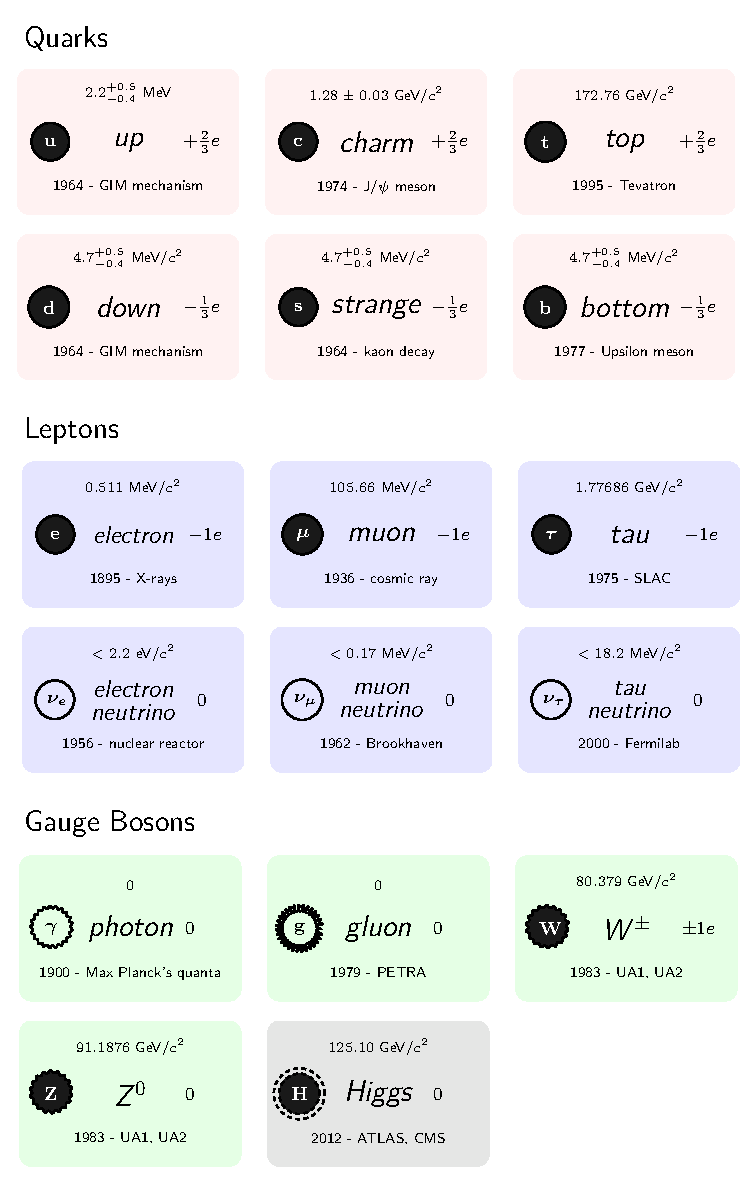
\includegraphics[width=0.90\textwidth]{\imgpath/SM.pdf}
\caption{Particle of the Standard Model, listed together with their mass, electric charge, and the  year and means of discovery (going clockwise from the top). VALUES NEED TO BE FIXED.}
\end{figure}

\section{Coordinate systems and kinematic observables}

Particles in HEP processes are described by their Lorentz-invariant four-vectors, $\bm{x} = (ct, x, y, z)$ and $\bm{p} = (E/c, p_x, p_y, p_z) = (E/c, \vec{\pt} , p_z)$, where $|\vec{\pt}| \equiv \sqrt{p_x^2+p_y^2}$. In LHC experiments, the coordinate system is defined such that the $x$-axis points in the direction of the centre of the LHC, and the $z$-axis points in the direction of the beam, as shown in Fig.~\ref{fig:intro:coordinates}. In addition to the standard Cartesian coordinates, two observables, $\varphi$ (azimuthal angle) and $\eta$ (pseudorapidity), are used to describe the position and momentum of particles relative to the interaction point, which is located at $x = y = z = 0$. Pseudorapidity is defined as a function of the polar angle $\theta$, where 
\begin{align}
\eta = -\ln(\tan(\theta/2)) \quad .
\end{align}
For high-momentum particles ($E \simeq pc$), pseudorapidity is an approximation of the rapidity relative to the beam, given by 
\begin{align}
y = \frac{1}{2} \ln \frac{E + p_z c}{E - p_z c} \quad .
\end{align}
Rapidity is a convenient quantity to use because it transforms additively under Lorentz boosts, unlike velocity. In these coordinates, the following relations hold:
\begin{align}
p_x = |\vec{\pt}| \cos \varphi \, , \quad \
p_y = |\vec{\pt}| \sin \varphi \, , \quad \
p_z = |\vec{p} \,| \sinh \eta \, .
\end{align}

\begin{figure}[H]
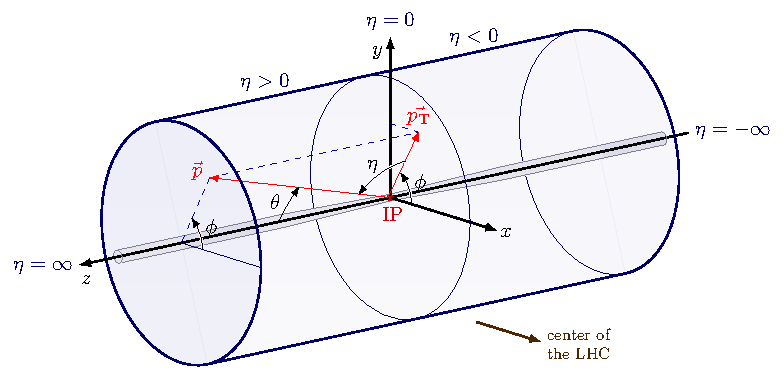
\includegraphics[width=0.85\textwidth]{\imgpath/coordinates.pdf}
\caption{Coordinate system of an LHC experiment, with the interaction point in the centre.}
\label{fig:intro:coordinates}
\end{figure}

\section{Quantum electrodynamics, electrons, and photons}

In many aspects, QCD is a very similar theory to the simpler and better explored theory QED. In QFT, dynamics of particles can be provided in terms of its Lagrangian density $\mathcal{L}$, from which equations of motions can be derived and which is also used to calculate interaction probabilites. The QED theory with a local U($1$) symmetry has its $\mathcal{L}_\mathrm{QED}$ defined as:

\begin{equation}
\mathcal{L}_\mathrm{QED} = \bar{\psi}(i \slashed \partial - m)\psi - \frac{1}{4}F_{\mu\nu}F^{\mu\nu} - e\bar{\psi}\slashed A \psi \quad ,
\end{equation}
where $\psi$ is the electron field with mass $m$ and electric charge $e$, $F_{\mu\nu}$ the electromagnetic field-strength tensor, and Feynman slash notation is employed. The first part describes the dynamics of the electron fields, the second part describes the dynamics of the electromagnetic field, and the last part describes the interaction of electrons and photons with a coupling strength $e$. Using Feynman diagrams, they can be visualised as:
\begin{figure}[H]
\adjustbox{valign=m}{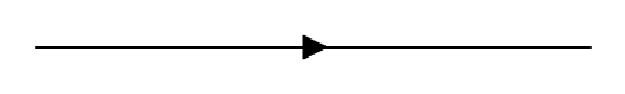
\includegraphics[width=0.19\textwidth]{\imgpath/qed1.pdf}}\hspace{1em}
\adjustbox{valign=m}{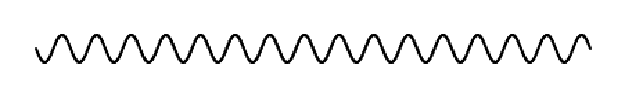
\includegraphics[width=0.19\textwidth]{\imgpath/qed2.pdf}}\hspace{1em}
\adjustbox{valign=m}{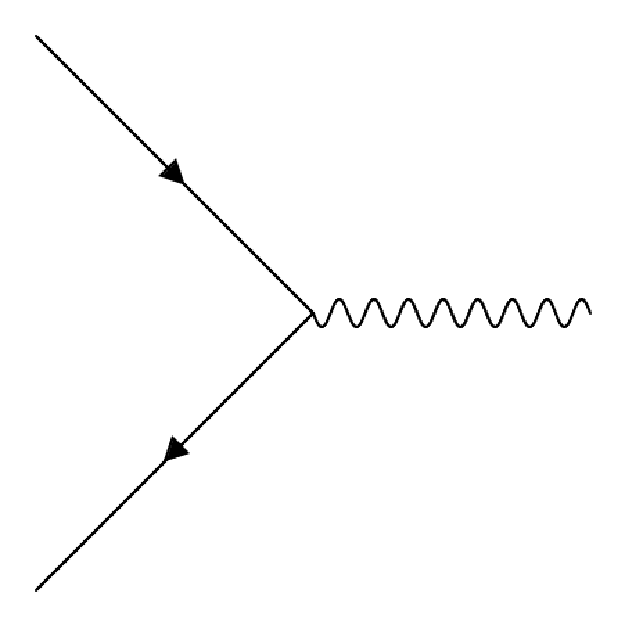
\includegraphics[width=0.19\textwidth]{\imgpath/qed3.pdf}}
\end{figure}

In QED interactions, each vertex depicted in the Feynman diagrams contributes to the probability of the process with a coefficient $\alpha$ (to the matrix elements as $\sqrt{\alpha}$, which is the coupling constant defined as $\alpha = e^2/4\pi$. This constant is generally small, which allows for interactions to be calculated using perturbation theory as an expansion series in $\alpha$. The contributions to the series correspond to different Feynman diagrams representing the possible interaction processes, and they are ordered in powers of $\alpha$ based on the complexity of the diagrams.

Contributions from higher orders, such as the electron loop depicted below, lead to ``screening" of the effective charge at large distances/small momenta, which makes the coupling constant dependent on the scale of the process $\mu$. For example, at low energies corresponding to atomic scales, $\alpha \approx 1/137$, but at scales of the $Z^0$ boson mass, $\alpha \approx 1/127$ \cite{fritzschFundamentalConstantsHigh2002}. The \textit{running} of this coupling is given by the $\beta$ function, $\beta(\alpha) \equiv \frac{\partial \alpha}{\partial \log \mu^2}$, and it can be calculated by quantifying the effective coupling strengths at various orders of perturbation theory and using renormalisation group tools \cite{delamotteHintRenormalization2004}, although renormalisation is a more general concept. In QED, the screening leads to a positive sign in $\beta$ calculated at lowest order, which means that when solving for $\alpha$ by integrating, $\alpha$ grows with energy scale\footnote{The scale at which QED eventually breaks down due to this increase is well above the Plack mass.}.

\begin{figure}[H]
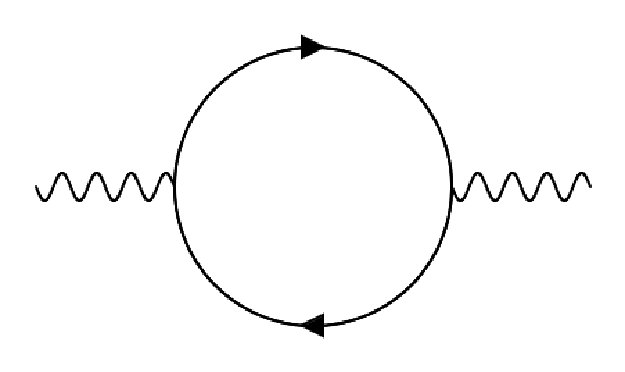
\includegraphics[width=.26\textwidth]{\imgpath/qedloop.pdf}
\end{figure}

Renormalisation is also used when calculating physical quantities where loop contributions lead to divergences, which are then absorbed into the parameters of the theory. The success of these procedures and the QED theory as a whole is validated by excellent prediction power for experimental measurements, such as the magnetic moment of an electron \cite{odomNewMeasurementElectron2006}.

\section{Quantum chromodynamics, quarks, and gluons}

In QCD, particles have an additional quantum number called colour charge: red, green, and blue. Thus, there are three quarks of each flavour and eight gluons mediating interactions between. Gluons also carry colour charges, which allows them to interact with each other, making the theory non-Abelian. The QCD Lagrangian is symmetric under local SU($3$) transformations and takes the shape of:

\begin{align}\label{eq:intro:lqcd}
\mathcal{L}_\mathrm{QCD} &= \sum_{f}^{n_f} \bar{\psi}_i^{(f)}(i \slashed D_{ij}-m_f \delta_{ij} ) \psi_j^{(f)} \, - \frac{1}{4} \sum_a^8 F^{\mu\nu}_a F_{\mu\nu}^a \quad , \\
D^\mu_{ij} &\equiv \partial^\mu \delta_{ij} + i g_s t^a_{ij}A^\mu_a \quad , \\
F^a_{\mu\nu} &\equiv \partial_\mu A^a_\nu - \partial_\nu A^a_\mu - g_s f_{abc} A^b_\mu A^c_\nu \quad ,
\end{align}
where $\psi$ are the quark fields of $n_f$ different flavours with mass $m_f$ and colour $i,j$, $D^\mu_{ij}$ the covariant derivative with the coupling strength $g_s$ and eight SU($3$) generators given by matrices $t^a_{ij}$, and $A_a^{\mu}$ are the gluon fields \cite{altarelliQCDPrimer2002}. Lastly, $F^a_{\mu\nu}$ is the field-strength tensor with $f_{abc}$ being structure constants. The Lagrangian now also contains terms with interactions between gluons. In the representation of Feynman diagrams, for the interactions, there is:
\begin{figure}[H]
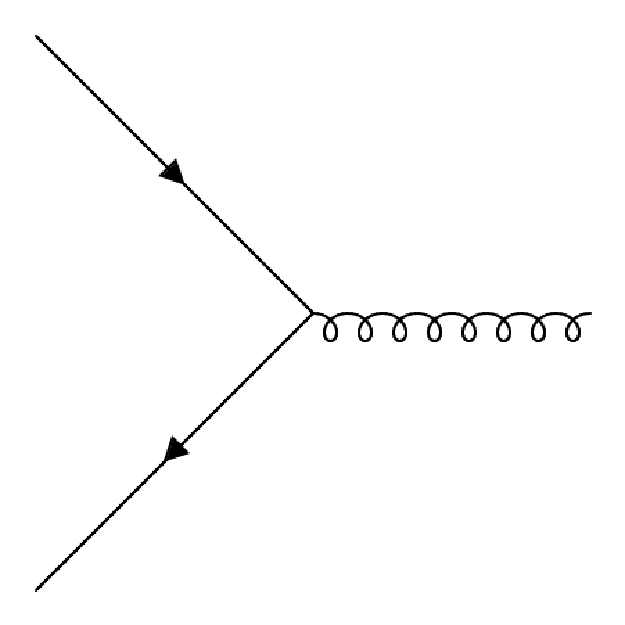
\includegraphics[width=0.19\textwidth]{\imgpath/qcd3.pdf}\hspace{1em}
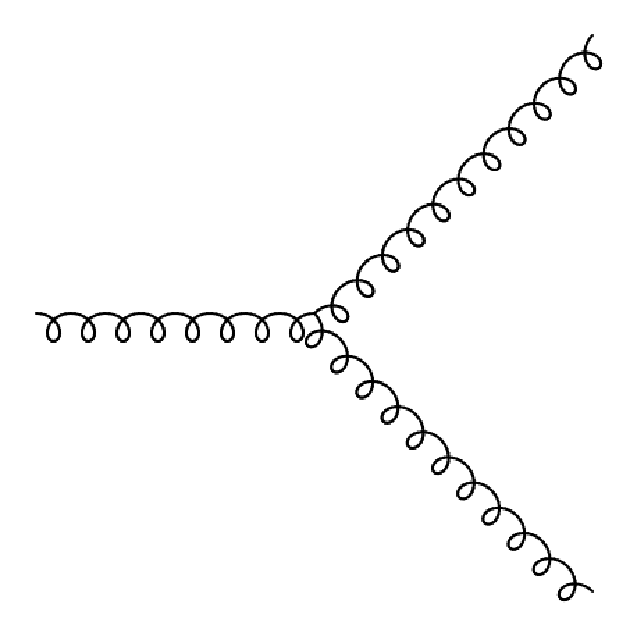
\includegraphics[width=0.19\textwidth]{\imgpath/qcd4.pdf}\hspace{1em}
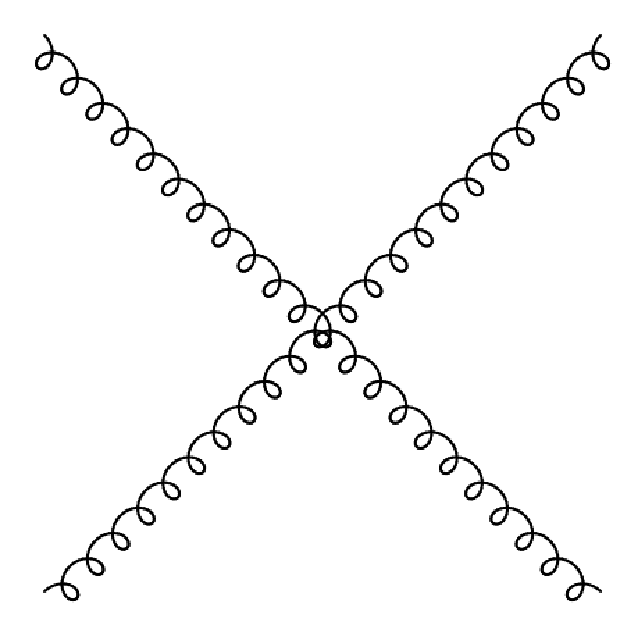
\includegraphics[width=0.19\textwidth]{\imgpath/qcd5.pdf}
\end{figure}

Similarly to the QED case, the strong coupling constant can be defined as $\alpha_s = g^2/4\pi$. However, when considering its modifications due to virtual corrections, in addition to the quark loop, there is also a gluon loop.:
\begin{figure}[H]
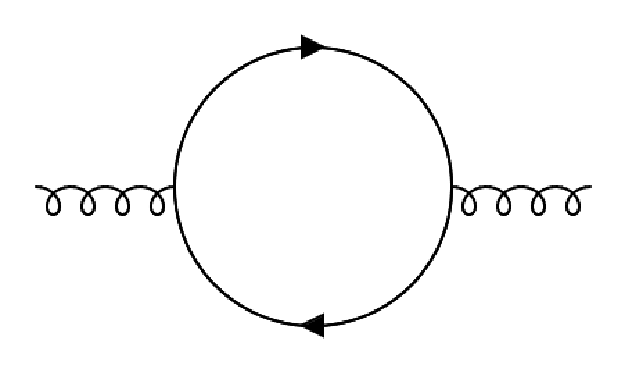
\includegraphics[width=0.26\textwidth]{\imgpath/qcdloop1.pdf}\hspace{2em}
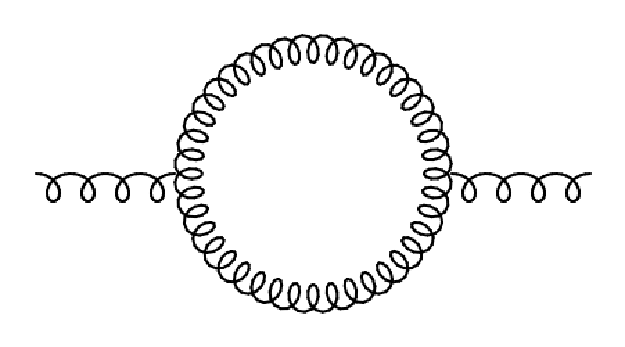
\includegraphics[width=0.26\textwidth]{\imgpath/qcdloop2.pdf}
\end{figure}

The gluon loop contributes to the $\beta$ function in an opposite and larger way than the quark loop, and so overall, there is an \textit{anti-screening} effect instead and a negative sign in the calculated one-loop $\beta$ function. The running of the coupling can be calculated as:
\begin{align}
\alpha_s (\mu) = \frac{1}{b_0 \log ( \mu^2 / \Lambda_\mathrm{QCD}^2 )} \quad ,
\end{align} 
where $b_0$ is a constant computed from the loop calculations, $b_0 = \frac{11-\frac{2}{3}n_f}{4\pi}$ \cite{politzerReliablePerturbativeResults1973}. The introduced $\Lambda_\mathrm{QCD}$ is a scale parameter of the theory corresponding to the energy where the coupling becomes infinite, and depends on the definition of $\alpha_s$ and the number of available quark flavours $n_f$ \cite{altarelliQCDPrimer2002}. It ranges between $200$ and $\mevcc{300}$ \cite{deurQCDRunningCoupling2016}.

From the running, it is evident that the coupling strength decreases with increasing energy, which is known as \textit{asymptotic freedom} \cite{politzerReliablePerturbativeResults1973,grossAsymptoticallyFreeGauge1973} and corresponds to the fact that strong interaction is short-ranged. On the other hand, at low values, $\alpha_s$ diverges, which is related to the fact that quarks are bound to hadrons -- \textit{quark confinement}. The evolution of $\alpha_s$ also limits the applicability of perturbation theory at low energy regimes; calculations from perturbative QCD (pQCD) are relevant at leading orders starting typically from $1-\gevcc{2}$. The measured $\alpha_s(\mu)$ is shown in Fig.~\ref{fig:intro:alpha}, and at scales of the $Z^0$ boson mass is approximately $0.1185 \pm 0.0006$ \cite{dissertoriDeterminationStrongCoupling2016, particledatagroupReviewParticlePhysics2022}.

\begin{figure}[H]
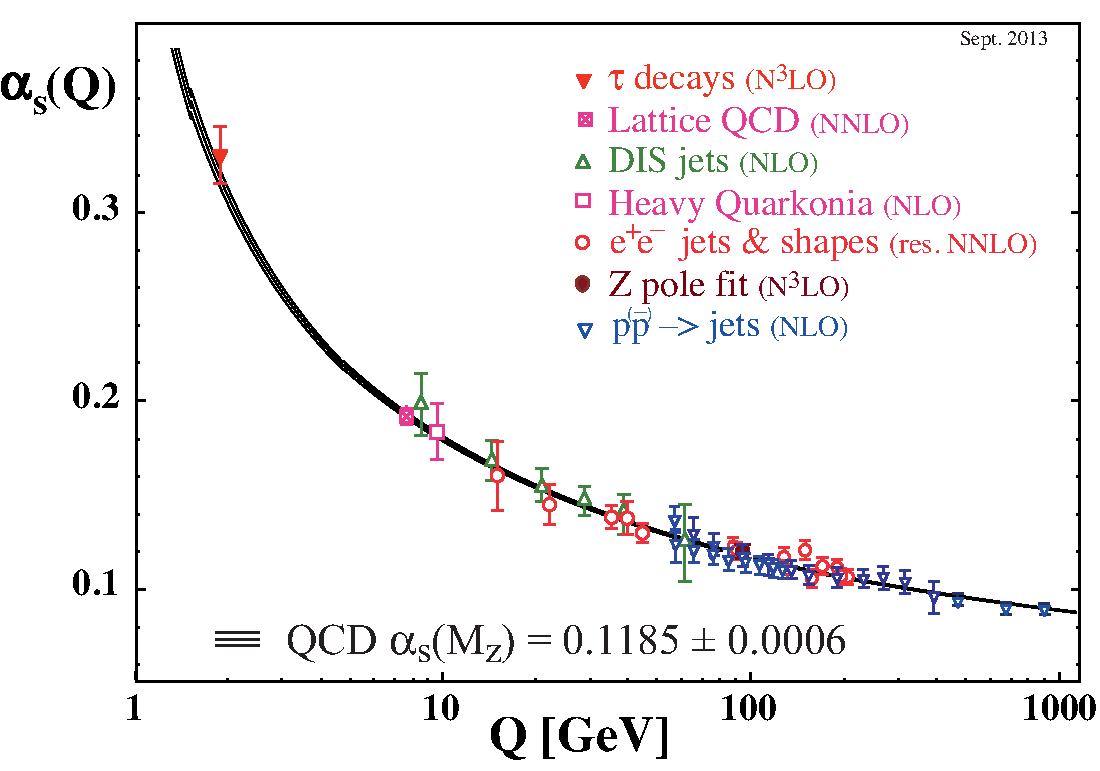
\includegraphics[width=0.55\textwidth]{\imgpath/alpha.pdf}
\caption{Strong coupling constant determined at different energy scales through various measurements and numerical calculations (data points) and compared with theoretical predictions from QCD. \cite{dissertoriDeterminationStrongCoupling2016}}
\label{fig:intro:alpha}
\end{figure}

\section{From partons to hadrons}

\subsection{Initial and Final State Radiation}

In QFT, charged particles are surrounded by a cloud of virtual particles, which can be thought of as fluctuations in the particle's field. For example, the electron state can be described as a superposition of the bare electron plus additional massless bosons:
\begin{align}
|\mathrm{e}\rangle_\mathrm{phys} = |\mathrm{e}\rangle + |\mathrm{e}\gamma\rangle + |\mathrm{e}\gamma\gamma\rangle + \ldots
\end{align}
and, at higher orders, pairs of virtual electrons. The fluctuations continuously form and recombine, with their lifetime depending on their energy and momentum. Specifically, the lifetime of a fluctuation with energy $\omega$ and transverse momentum $k_\mathrm{T}$ can be approximated as:
\begin{align}
\tau \approx \frac{\omega}{k_\mathrm{T}} \quad .
\end{align}
This implies that fluctuations with smaller-$k_\mathrm{T}$ live longer. \cite{prestelParticlePhysicsPhenomenology}

As illustrated in Fig.~\ref{fig:intro:isrfsrsketch}, the coherent mixed state of the bare charge and the field fluctuations can be disturbed by the presence of an interaction. Intuitively, this interaction can change the energy and momentum of the fluctuations, their formation and recombination, and lead to the emission of radiation in two ways:
\begin{enumerate}
\item a fluctuation is kicked on-shell by the interaction and part of the field continues in its original direction, which leads to Initial State Radiation (ISR);
\item as a result of the field of the scattered particle rearranging itself , which can be a source of Final State Radiation (FSR).
\end{enumerate}

In both of the cases, a larger momentum transfer implies more radiation. \textit{For hard, wide angle emissions, cross sections can be calculated perturbatively at fixed orders}. 

Soft and collinear emissions, however, lead to infra-red divergences ($\propto \frac{1}{\omega}$,$\propto \frac{1}{k_\mathrm{T}^2}$) and thus, need to be factorised away from the amplitudes or the cross sections and then described using resummation techniques. Without any emissions, the probabilities of finding electrons and photons of fractional momentum $x$ with respect to the whole system are:
\begin{align}
f_\mathrm{e} (x) = \delta (1-x) \, , \quad \ f_\gamma(x) = 0 \, ,
\end{align}
When considering the emissions above some scales parametrised by the resolution parameter $Q^2$, these probabilities, however, evolve according to the DGLAP equation \cite{altarelliAsymptoticFreedomParton1977} :
\begin{align}
\label{eq:intro:dglap}
\frac{\partial}{\partial\ln Q^2}
\begin{pmatrix}
f_e(x, Q^2)\\
f_{\gamma}(x, Q^2)
\end{pmatrix}
&= \frac{\alpha_\mathrm{em}}{2\pi}
\int_x^1 \frac{dz}{z}
\begin{pmatrix}
P_{ee}(z) & P_{e\gamma}(z)\\
P_{\gamma e}(z) & P_{\gamma\gamma}(z)
\end{pmatrix}
\begin{pmatrix}
f_e\left(\frac{x}{z}, Q^2\right)\\
f_{\gamma}\left(\frac{x}{z}, Q^2\right)
\end{pmatrix} \quad ,
\end{align}
where $P_{ij}(z)$ are the splitting probability functions of a particle $i$ emitting a particle $j$.

In QCD, the behaviour is analogous, with $\alpha_\mathrm{em} \rightarrow \alpha_s$, $e\rightarrow q$, and $\gamma \rightarrow g$. \cite{prestelParticlePhysicsPhenomenology}

\begin{figure}[H]
\subfloat[][]{\adjustbox{valign=m}{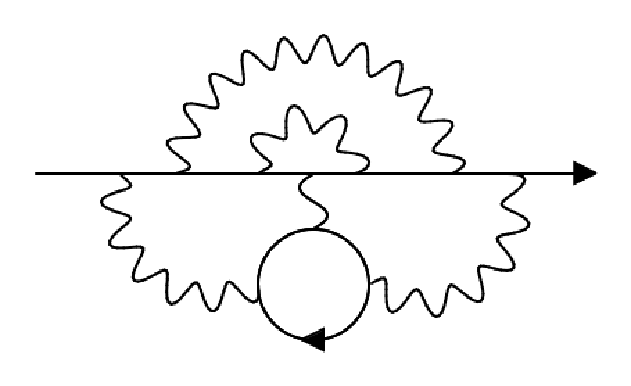
\includegraphics[width=.240\textwidth]{\imgpath/eisr1.pdf}}\adjustbox{valign=m}{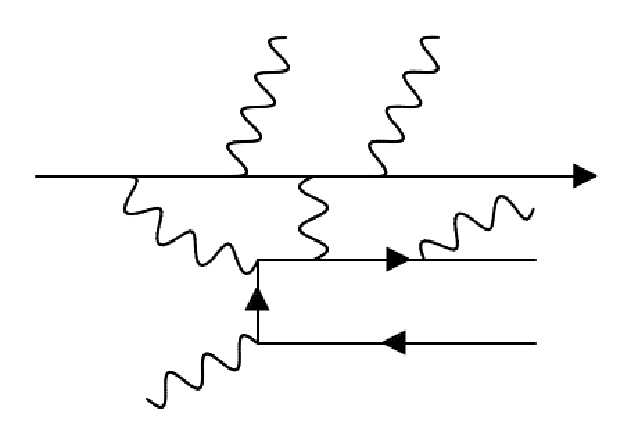
\includegraphics[width=.240\textwidth]{\imgpath/eisr22.pdf}}}
\subfloat[][]{\adjustbox{valign=m}{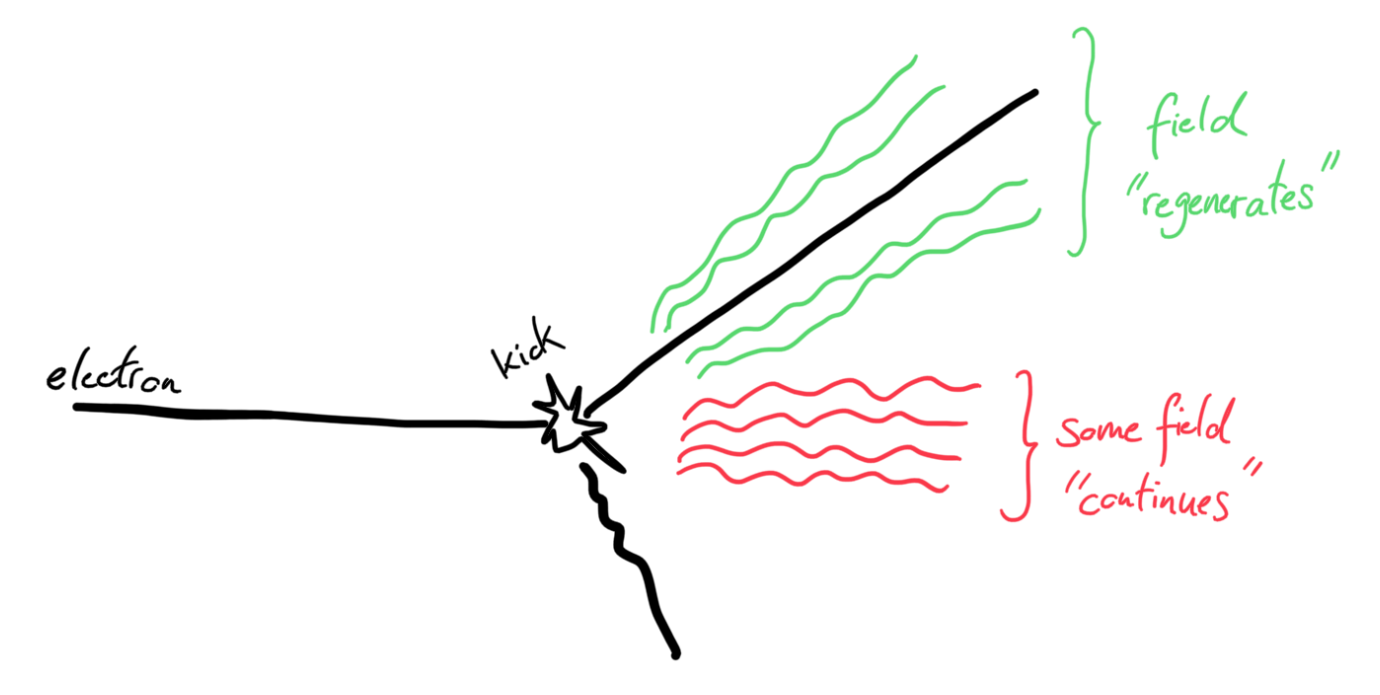
\includegraphics[width=.480\textwidth]{\imgpath/isrfsr2.png}}}
\caption{\textbf{(a)} Illustration of the field fluctuations before and after the state coherence gets disturbed by an external actor. \textbf{(b)} Illustration of emmisions of radiation in a scattering process.}
\label{fig:intro:isrfsrsketch}
\end{figure}

\subsection{Factorisation theorem}

The evolution equation (\ref{eq:intro:dglap}) implies that the probabilities of observing emissions with a fractional momentum $x$ depend on the resolution $Q^2$. In QCD, 
\begin{enumerate}
\item when applied to the initial state, they are known as parton distribution functions (PDFs) and determine the probabilities of finding partons\footnote{Partons refer to the valence quarks, sea quarks, and gluons inside hadrons.} in the composite hadronic state. 
\item When applied to the final state, they are called fragmentation functions, and determine the probabilities of measuring fragments of the outgoing particles.
\end{enumerate}

This leads to the factorisation theorem \cite{collinsFactorizationHardProcesses2004} for processes involving collisions of two hadrons, which separates the perturbatively calculable partonic cross section from the non-perturbative partonic evolution and hadronisation. The theorem can be expressed as follows:
\begin{align}\label{eq:intro:facto}
\sigma = f_i^A(x_i,\mu_F)f_j^B(x_j,\mu_F) \otimes \hat{\sigma}_{ij\to n}(\mu_F,\mu_R) \otimes D_{n \to n'} \, .
\end{align}
Here, $i$ and $j$ are the initial partons, $\hat{\sigma}_{ij\to n}$ is the partonic cross section, $D_{n \to n'}$ is the process-specific fragmentation function for evolving the partons $n$ into the particles' final state $n'$, and $\mu_F$ and $\mu_R$ are the factorisation and renormalisation scales, respectively. The factorisation scale, $\mu_F$, determines the scale below which the emissions are absorbed into the PDFs. The theorem is depicted in Fig.~\ref{fig:intro:factorisation}.

\begin{figure}[H]
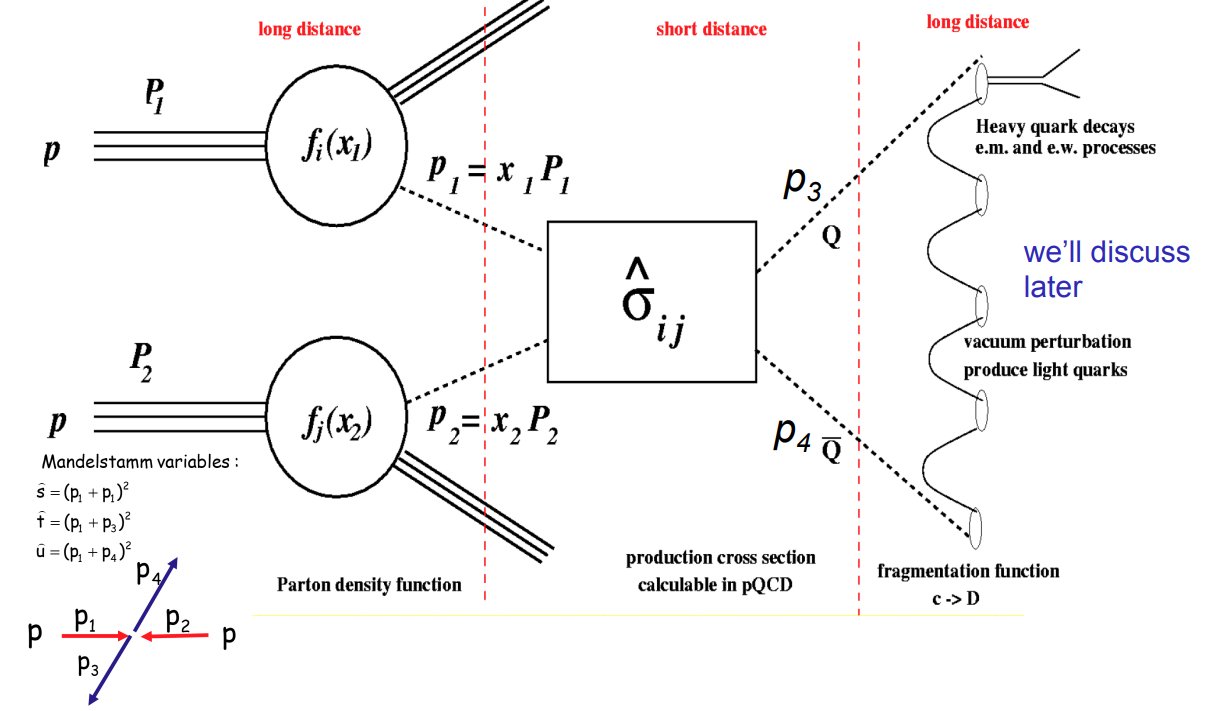
\includegraphics[width=0.65\textwidth]{\imgpath/factorisation.png}
\caption{Illustration of the factorisation theorem. (NEEDS TO BE REMADE).}
\label{fig:intro:factorisation}
\end{figure}

\subsection{Parton distribution functions}

The PDFs defining the probabilities of finding quarks and gluons in nucleons can be determined experimentally at hadron-electron colliders such as HERA \cite{cooper-sarkarExtractionProtonParton2008}. They are determined from measurements of deep inelastic scatterings in a range of energies and momentum transfers. They are displayed in Fig.~\ref{fig:intro:pdfs} as a function of the fractional momentum $x$ (also called Bj\"orken $x$). 

According to collider kinematics, $x \propto \frac{1}{\sqrt{s}e^y}$, therefore, the partonic composition of ultra-relativistic hadrons is dominated by gluons. Following unitarity principles and BK evolution equation \cite{marquetBalitskyKovchegovEquationFull2005}, it is expected that gluons start recombining and the gluonic content saturates as $x\rightarrow0$. This is actively reseached \cite{starcollaborationEvidenceNonlinearGluon2022}, however, not directly measured yet. Additionally, it should be noted that in ultra-relativistic heavy nuclei, the partons are modified in the contracted nuclear environment and the PDFs are referred to as nPDFs.

\begin{figure}[H]
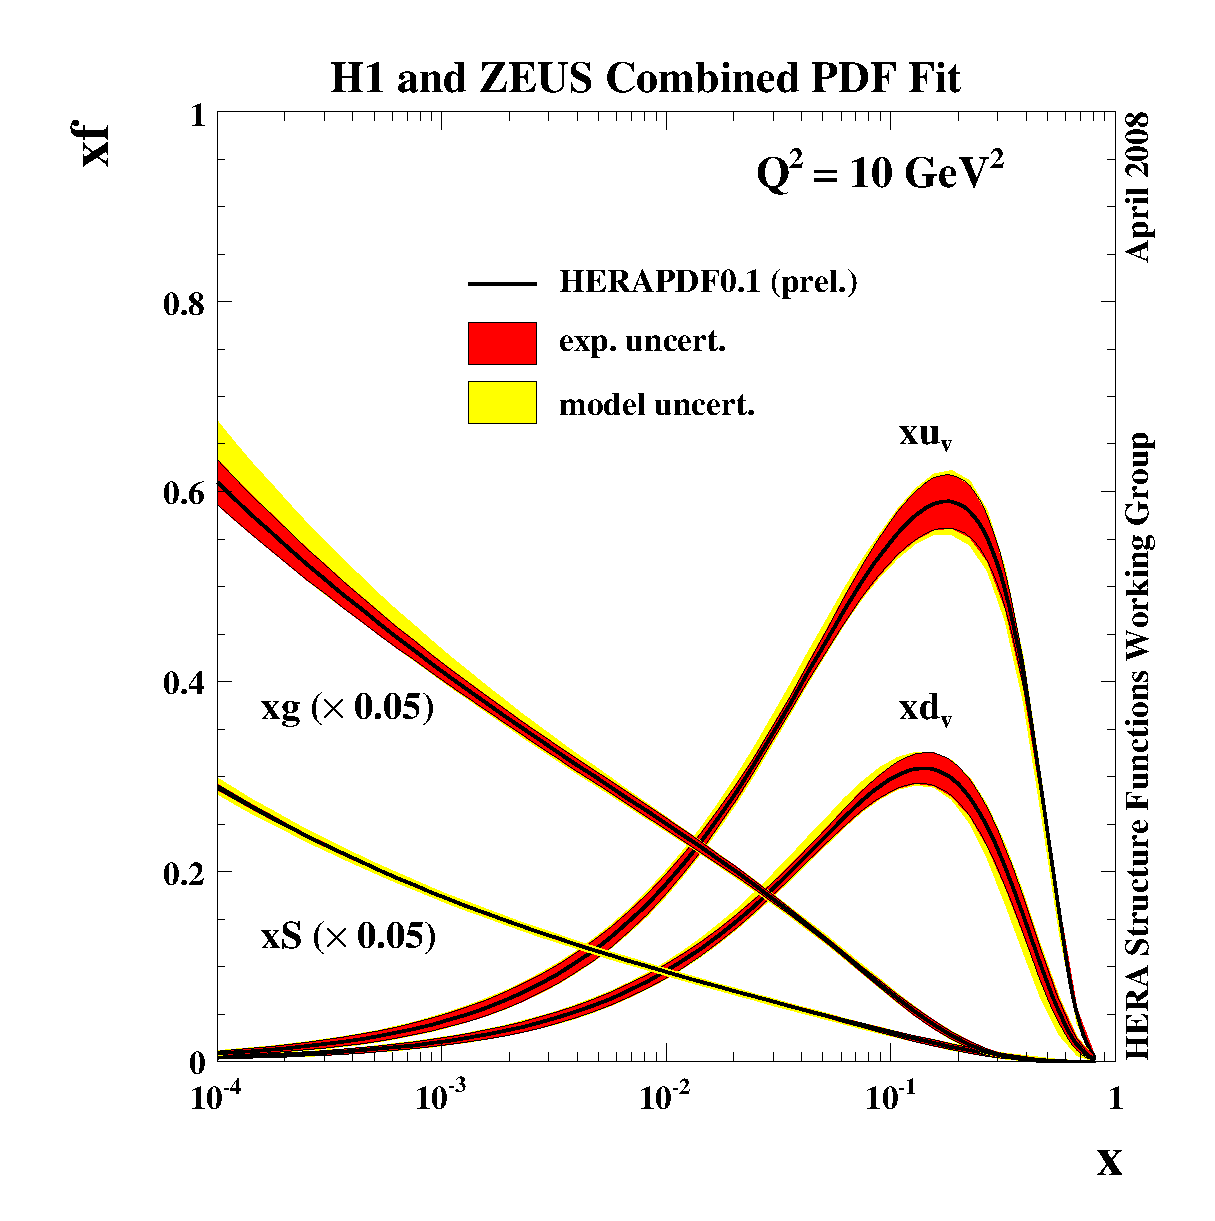
\includegraphics[width=0.4\textwidth]{\imgpath/pdf.eps}
\caption{Parton distribution functions determined in ep scatterings at HERA as a function of the fractional momentum for the up, down, sea quarks, and gluons. \cite{cooper-sarkarExtractionProtonParton2008}}
\label{fig:intro:pdfs}
\end{figure}

\subsection{Parton fragmentation and the Lund string}

After the scattering process, the produced partons continue to fragment by emitting more partons in a process called the parton shower. Since the coupling strength in QCD increases with decreasing the energy scale of the splitting, this leads to the production of many soft, collimated emissions known as jets. The partonic evolution continues until the virtuality of the partons reaches the hadronization scale ($\approx \Lambda_\mathrm{QCD}$). There are multiple frameworks within QCD to describe the evolution of partons into their final state, such as using the DGLAP equations or the so-called dipole formalism.

Once the partonic final state is reached, the partons hadronise into the observable mesons and baryons. The hadronisation process is not calculable in QCD and requires phenomenological models to describe it. One such model is the Lund string model \cite{ferreres-soleSpaceTimeStructureHadronization2018}, which describes hadronisation as the breaking of a color string between the quarks in the final state. In this model, the energy stored in the color string is converted into the mass of new hadrons.

According to confinement, hadronisation should involve at least two partons with complementary colours. In QCD, the $q\bar{q}$ potential takes the shape of
\begin{align}\label{eq:intro:qqpot}
V_{q\bar{q}} \approx - \frac{4}{3}\frac{\alpha_s \hbar c}{r} + \kappa r \quad ,
\end{align}
where $\kappa$ is a parameter with value around $1 \mathrm{GeV} /\mathrm{fm}$. In the non-perturbative regime (long distances), the potential is dominated by the linear part, which is reminiscent of a system bound by a string with tension $\kappa$. This is taken advantage of by the Lund string model -- a $q$ and $\bar{q}$ pair separated by distance $\Delta x$ is bound by a color field (string) with energy $\kappa \Delta x$. 

If the $q$ and $\bar{q}$ continue separating as a result of the scattering, the energy stored in the color field increases. At some point, it can become energetically favourable to produce a new $q\bar{q}$ pair out of vacuum, which is a quantum mechanics tunnelling phenomenon characterised by the probability:
\begin{align}
\frac{\mathrm{d}P}{\mathrm{d}m_\mathrm{T}} \propto \exp \left( -\frac{\pi m_\mathrm{T}^2}{\kappa} \right) \quad ,
\label{eq:intro:tunnel}
\end{align}
where $m_\mathrm{T}$ is the transverse mass of the produced quarks. Otherwise, the $q\bar{q}$ system starts contracting and oscillates with a period $T = 2 E_\mathrm{kin}/\kappa$, where $E_\mathrm{kin}$ is its maximum kinetic energy. The produced $q$ and $\bar{q}$ then connect by new color fields to the original pair. This process repeats itself resulting in a cascade of many $q\bar{q}$ pairs connected by many color strings. In this description, baryons can also be created by double tunnelling of a $qq\overline{qq}$ pair. The process is illustrated in Fig.~\ref{fig:intro:lundstring}.

\begin{figure}[H]
\subfloat[][]{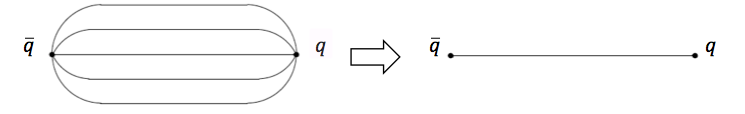
\includegraphics[width=.330\textwidth]{\imgpath/tubelike.png}}
\subfloat[][]{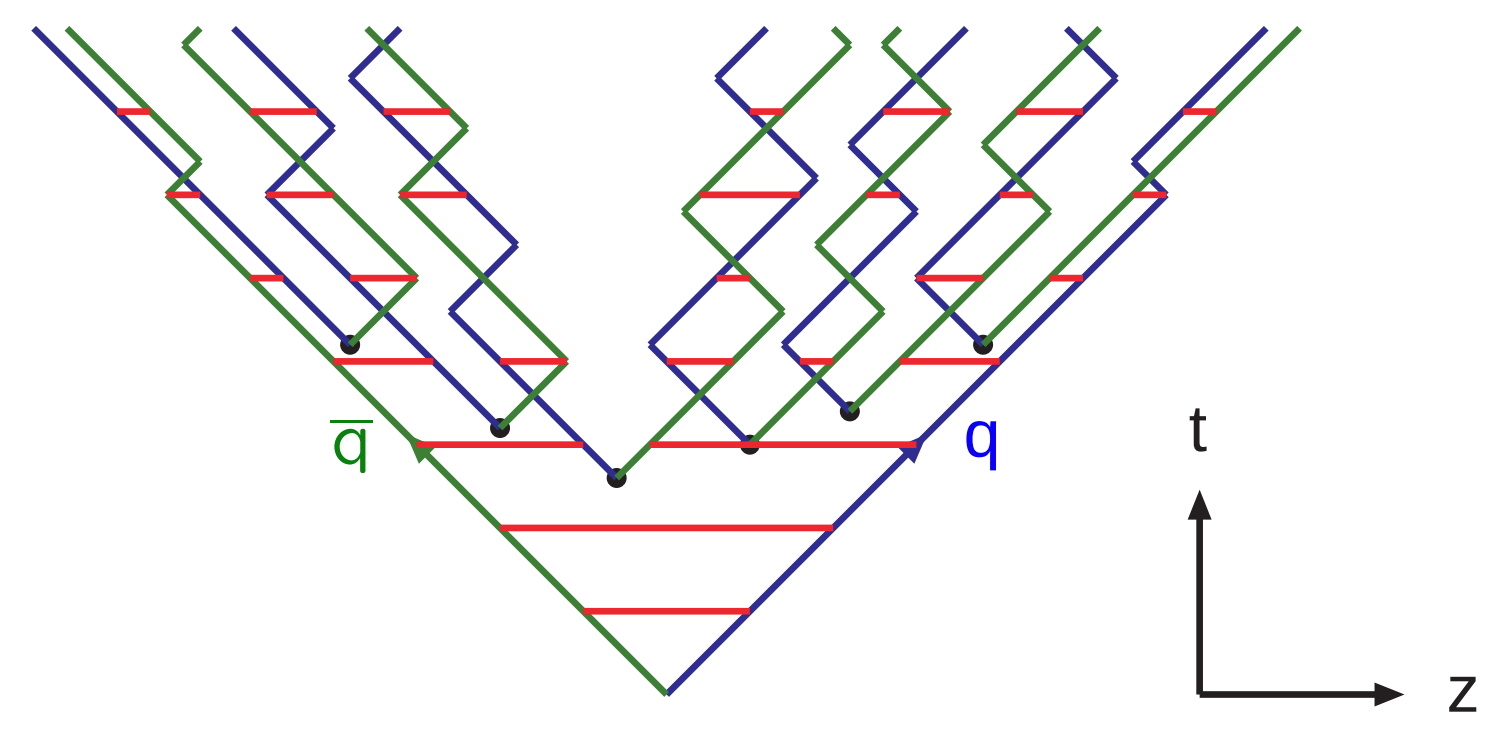
\includegraphics[width=.330\textwidth]{\imgpath/lundstring.png}}
\subfloat[][]{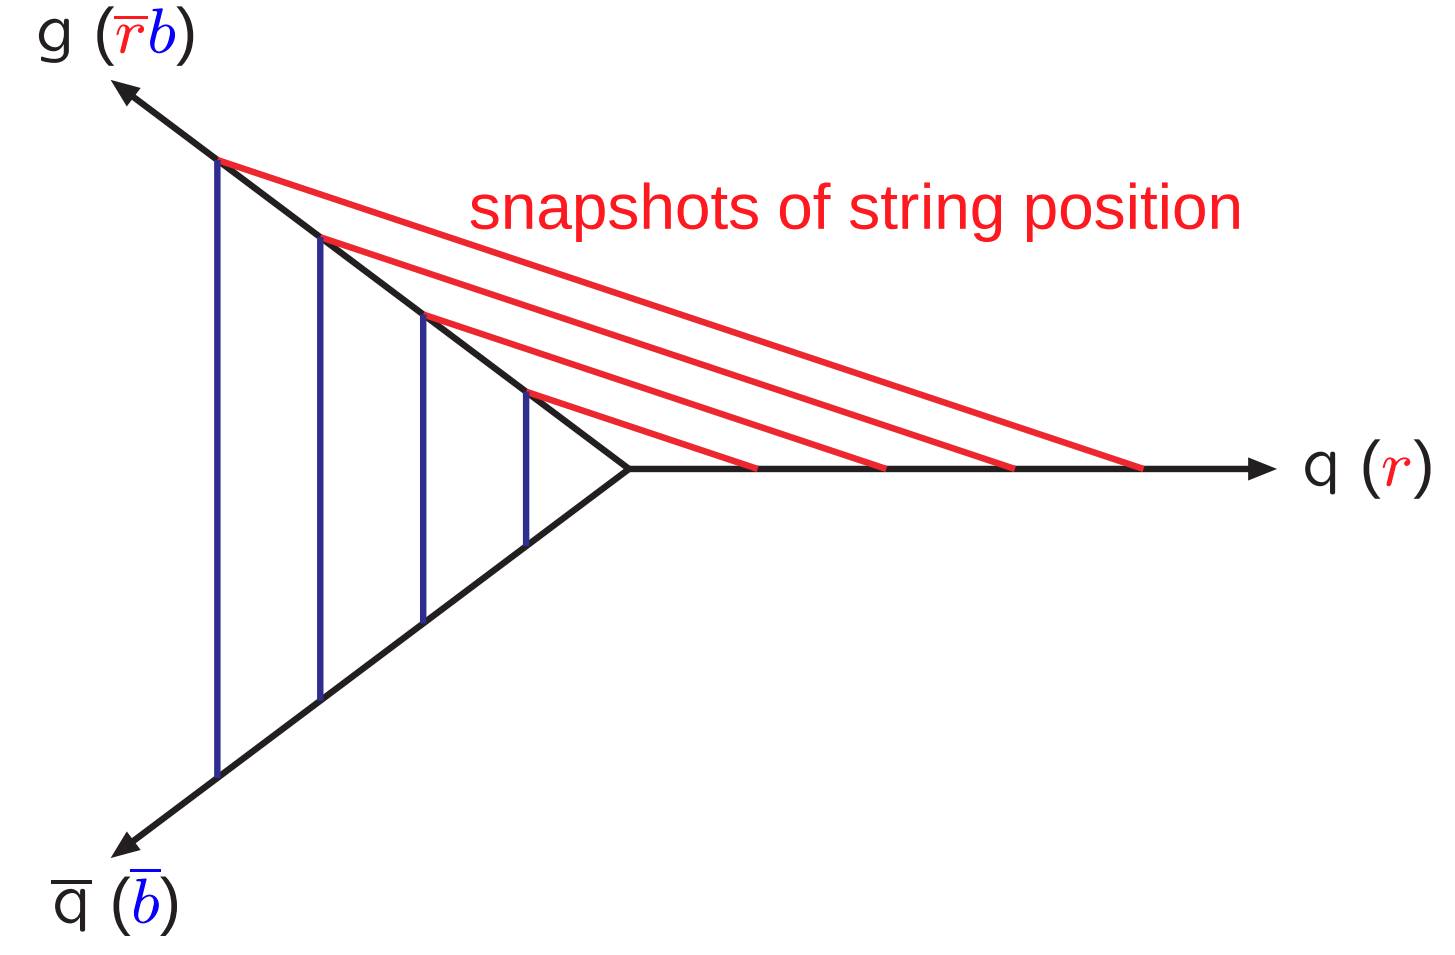
\includegraphics[width=.330\textwidth]{\imgpath/lundgluon.png}}
\caption{\textbf{(a)} Illustration of the color field between two quarks and its simplified representation with a string  \cite{ferreres-soleSpaceTimeStructureHadronization2018}. \textbf{(b)} Illustration of the string splitting by producing new $q\bar{q}$ in the $t-z$ plane \cite{ferreres-soleSpaceTimeStructureHadronization2018}. \textbf{(c)} Visualisation of the treatment of gluons in the Lund string model \cite{sjostrandQCDBSMPYTHIA2011}.}
\label{fig:intro:lundstring}
\end{figure}

Equation \ref{eq:intro:tunnel} also implies that production of strange quarks is suppressed by a factor of 
\begin{align}\label{eq:intro:rho}
\rho = \exp \left( -\frac{\pi (m^2_s - m^2_{u,d})}{\kappa} \right) \quad .
\end{align}
This parameter is typically tuned to data, as substituting constituent ($m_s \approx \gevcc{0.5}$, $m_{u,d} \approx \gevcc{0.33}$) versus current masses ($m_s \approx \gevcc{0.1}$, $m_{u,d} \approx 0$) leads to considerable differences underestimating and overestimating data, respectively.

For a $q\bar{q}g$ system, in this model, the gluon connects to the quark and antiquark and is effectively treated as a ``kink" on the color field, adding energy and momentum to the $q\bar{q}$ string (stretching it in its direction), as visualised in Fig.~\ref{fig:intro:lundstring}.

It should be noted that in the paradigm of AA collisions, hadron production can be alternatively modelled by hadronisation at the QGP's phase boundary by \textit{coalescing} free quarks.
%CooperFrye freezeout

%%!!!!TBA a sentence about the actual hadronisation.

\section{Multiple partonic interactions}

Results from $\mathrm{Sp\bar{p}S}$ in the 1980s sparked motivations for considering interactions of multiple partons between the two composite protons. For example, the AFS experiment observed an abundance of 4-jet events, displayed in Fig.~\ref{fig:intro:afs4jet}, that could not be explained by calculations considering a double gluon bremsstrahlung from a single partonic scattering\cite{akessonDoublePartonScattering1987}. Furthermore, UA5 measurements studying energy dependence of multiplicity distributions P(\Nch) saw the so-called KNO scaling\cite{kobaScalingMultiplicityDistributions1972}, where P(\Nch)/\meanNch does not depend on energy, but revealed a broadening in high-multiplicity events with increasing $\sqrt{s}$\cite{alnerScalingViolationFavouring1984,ansorgeChargedParticleMultiplicity1989}, which was not reproducible in the context of \Nch being produced from a single string \cite{sjostrandDevelopmentMPIModelling2017}. This further suggested the presence of multiple production sources.

\begin{figure}[H]
\subfloat[][]{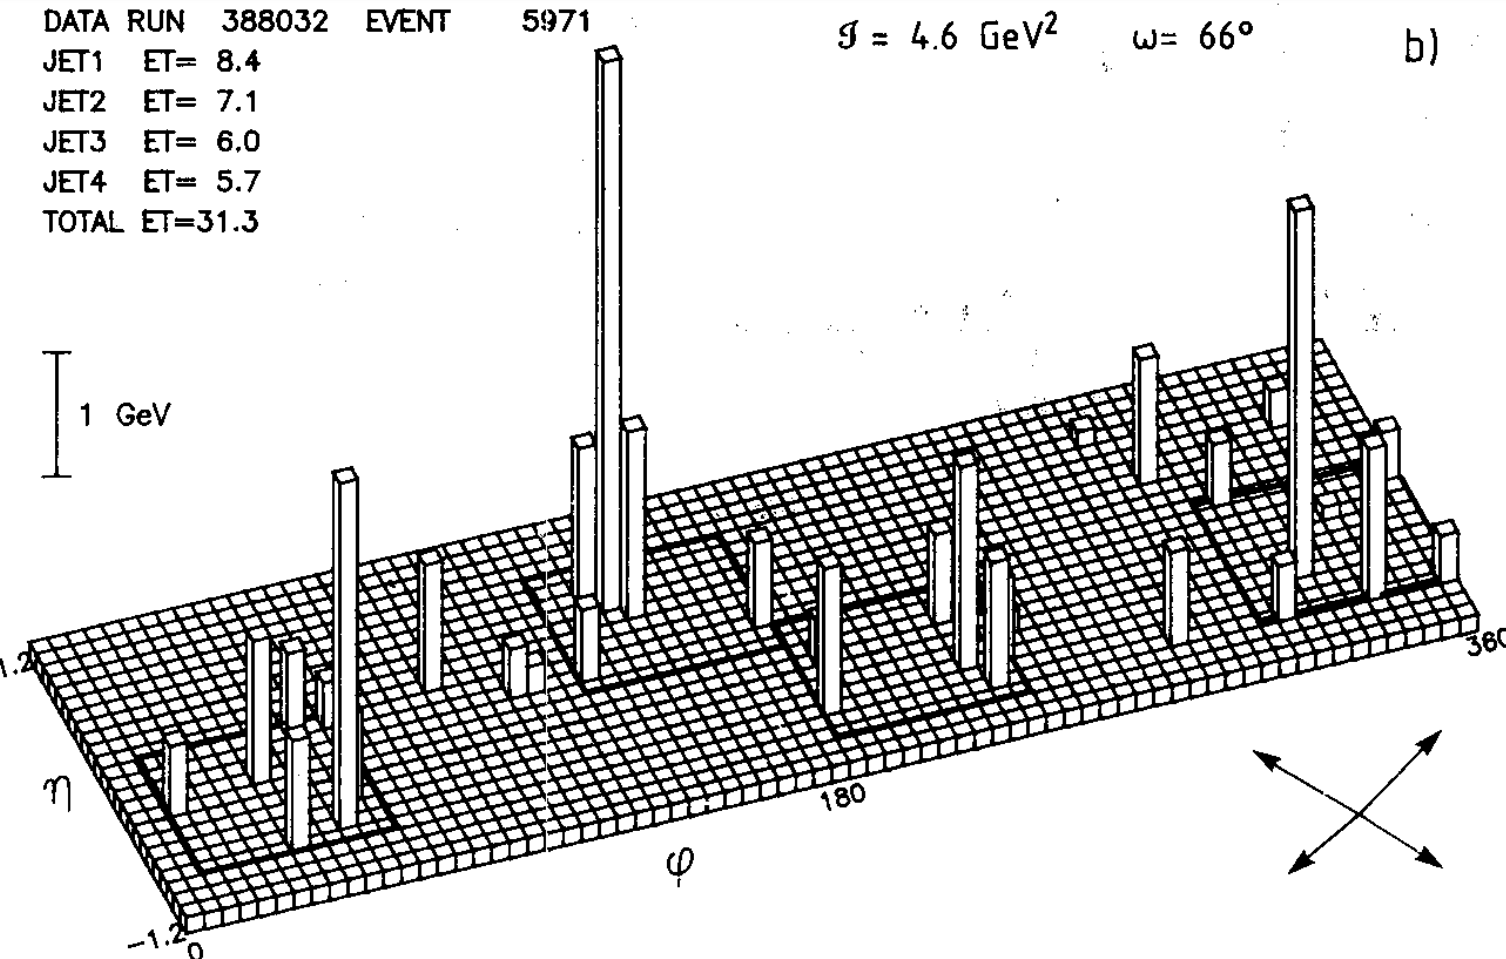
\includegraphics[width=.520\textwidth]{\imgpath/afs4jet.png}} 
\subfloat[][]{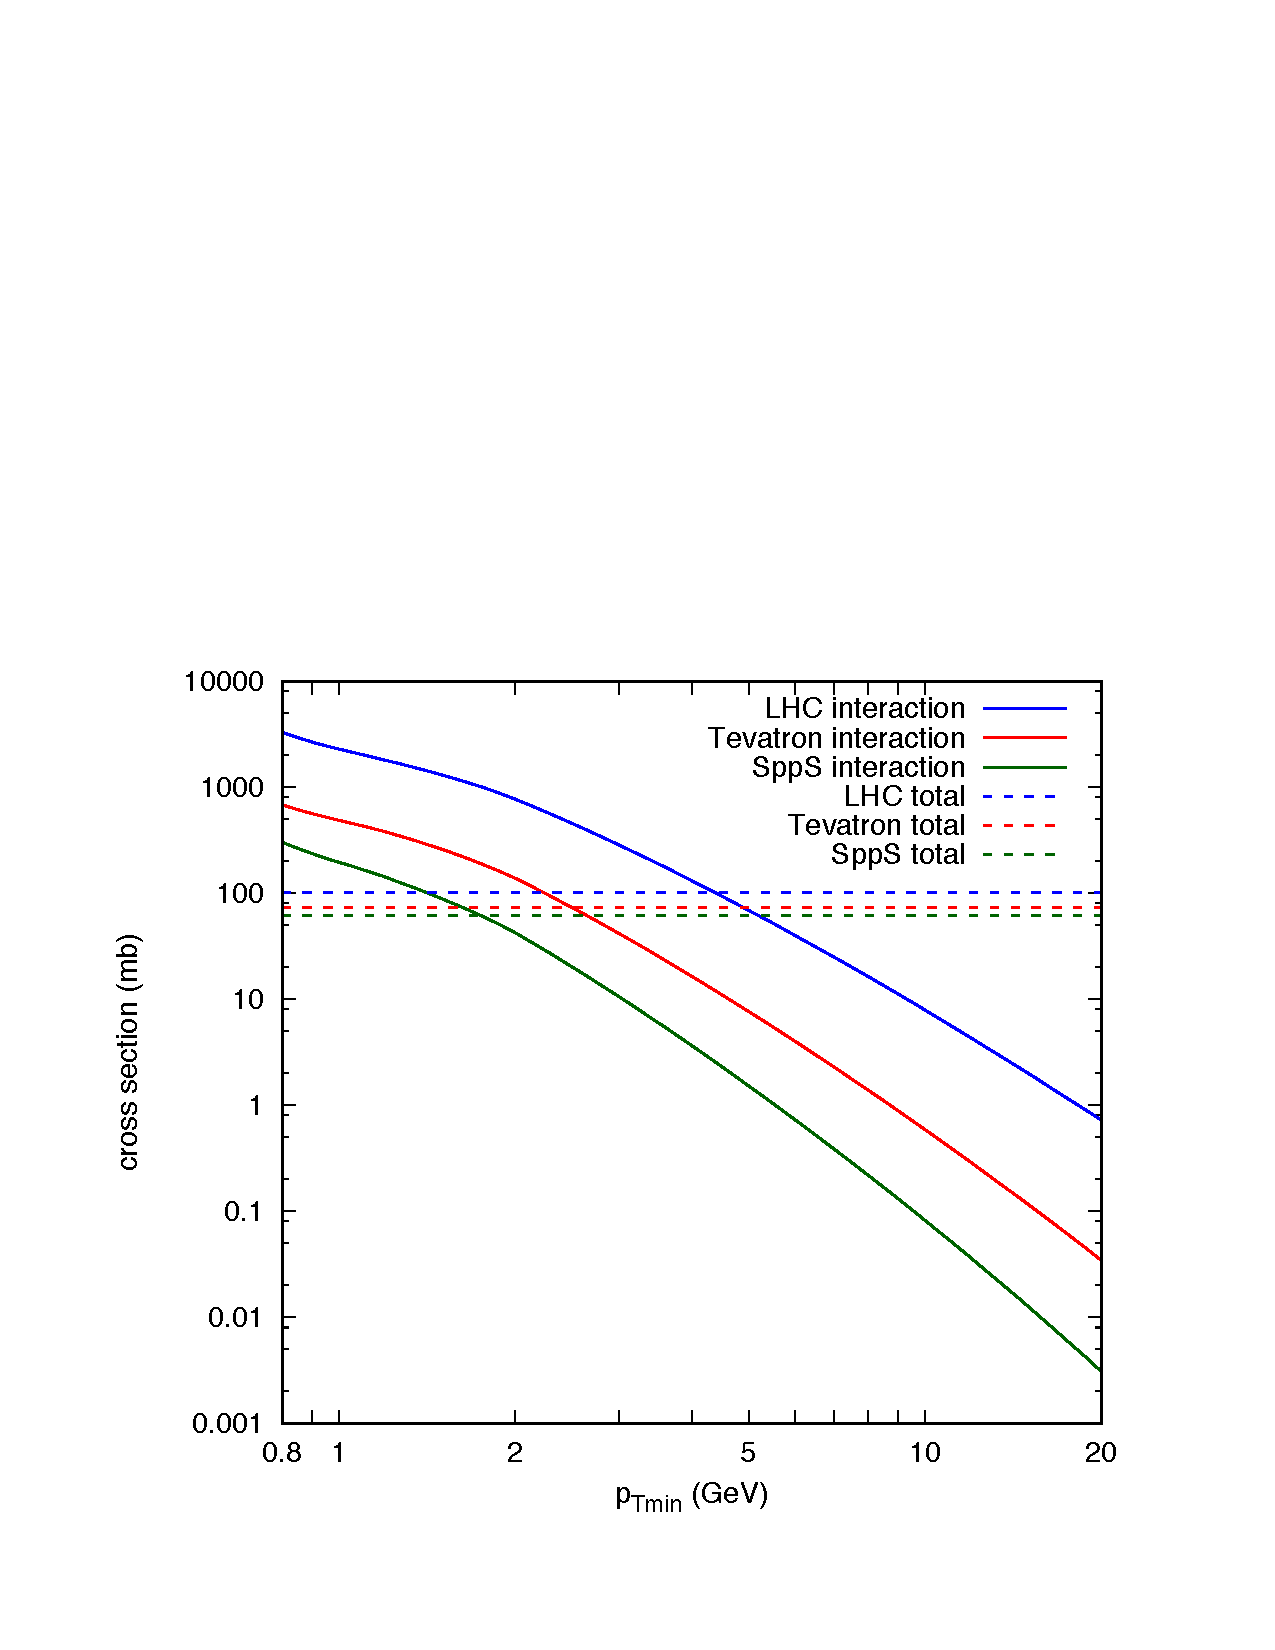
\includegraphics[width=.380\textwidth]{\imgpath/sigmampi.pdf}}
\caption{\textbf{(a)} Event display of an event with a 4-jet, where the pillars correspond to transverse energy deposits. \cite{akessonDoublePartonScattering1987} \textbf{(b)} Dependence of the integrated parton-parton cross section on the cutoff parameter $k_{\perp \mathrm{min}}$ for $\mathrm{Sp\bar{p}S}$ at \sppt{0.63}, Tevatron at \sppt{1.96}, and the LHC at \sppt{13}, modelled with Pythia. \cite{sjostrandDevelopmentMPIModelling2017}}
\label{fig:intro:afs4jet}
\end{figure}

These findings prompted further development of Regge theory and approaches that incorporated multiple pomerons, which were successful in describing the \Nch distributions. However, this approach is fully decoupled from descriptions of the perturbative primary scattering. Subsequently, much of the phenomenology related to multiple partonic interactions was developed within the framework of the Pythia MC event generator, which is discussed individually in Chapter~\ref{chap:colls} \cite{sjostrandDevelopmentMPIModelling2017}. However, nowadays, the relevance of the concept of MPIs in hadronic collisions extends beyond this generator. A scattering with double partonic interactions is illustrated in Fig.~\ref{fig:intro:dps}.

\begin{figure}[H]
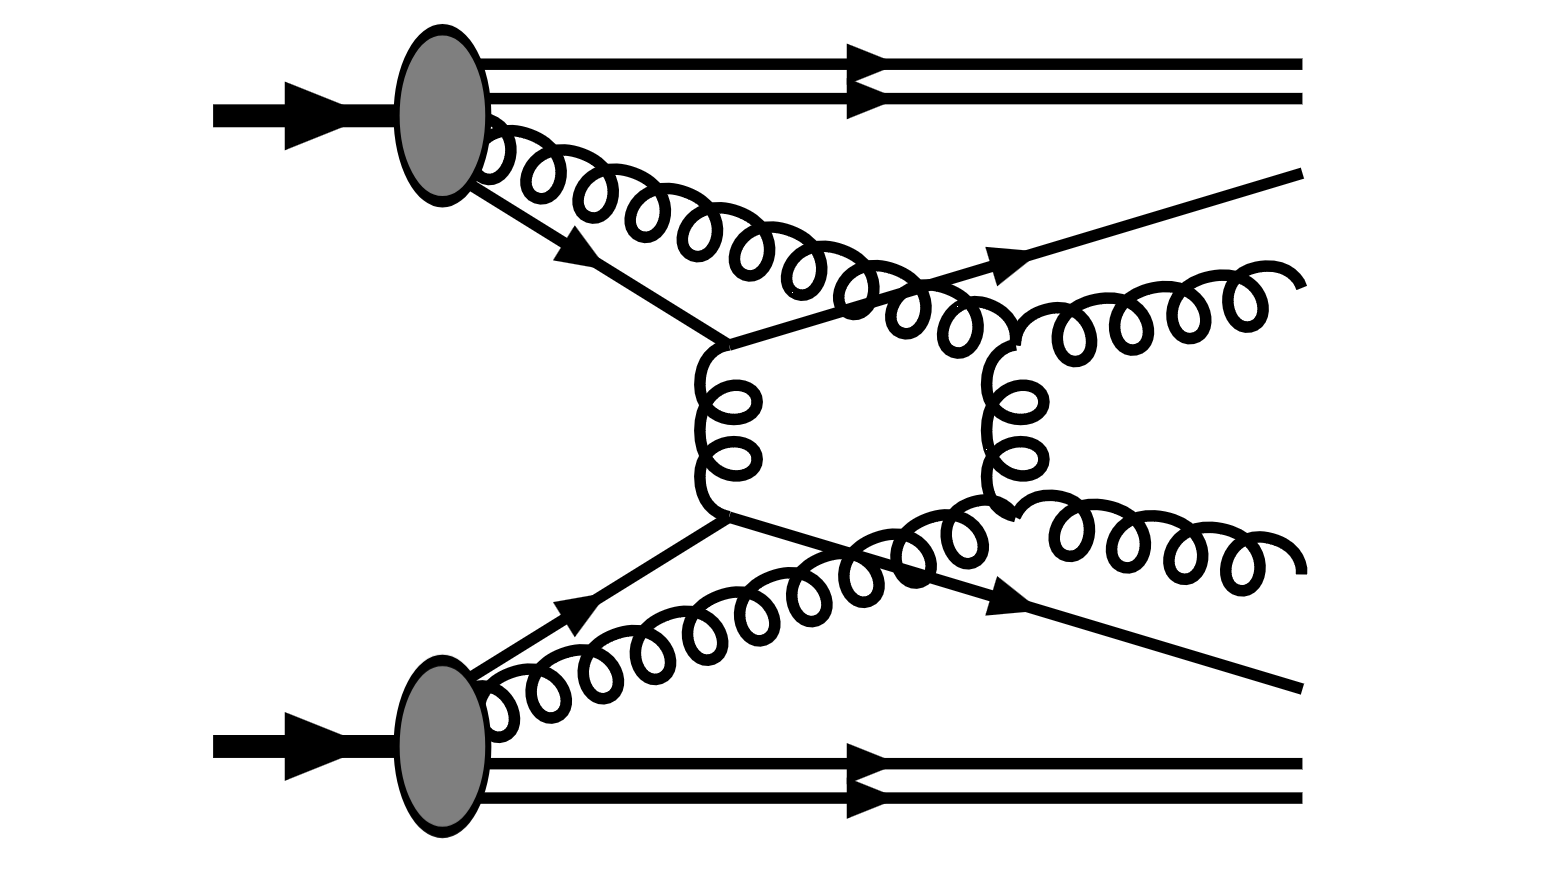
\includegraphics[height=7em]{\imgpath/dps.png}
\caption{Diagram showing a double partonic interaction, a case of $\nmpi=2$. \cite{prestelParticlePhysicsPhenomenology}}
\label{fig:intro:dps}
\end{figure}

In the Pythia approach, MPI are treated as additional perturbative scatterings. In QCD, the $2\to2$ cross section (dominated by the gluon exchange t-channel) diverges as $\propto \alpha^2_S(k_{\perp}^2)/k_{\perp}^4$, so a cutoff parameter $k_{\perp\mathrm{min}}$ must be introduced, and using (\ref{eq:intro:factorization}) leads to:
\begin{align}
\frac{d\sigma}{dk_{\perp}^2} &= \sum_{ij}\int dx_1 dx_2 f_i(x_1,\mu_F^2)f_j(x_2,\mu_F^2) \frac{d\hat{\sigma}^H_{ij}}{dk_{\perp}^2} \, , \\
\sigma_{\text{int}}(k_{\perp\text{min}}) &= \int_{k_{\perp\text{min}}^2}^{s/4} \frac{d\sigma}{dk_{\perp}^2}dk_{\perp}^2 \, .
\end{align}
The choice of cutoff can be tuned to experimental data, and for the $\mathrm{Sp\bar{p}S}$ energy of \sppg{630}, a value of around \gevc{1.6} was typical \cite{sjostrandDevelopmentMPIModelling2017}. The dependence of this parton-parton scattering cross section is shown in Fig.~\ref{fig:intro:afs4jet}.

The total pp cross-section, which is on the order of $100$~mb at \sppt{13}, is given by
\begin{align}
\sigma_{\mathrm{pp}} &= \sigma_{\mathrm{elastic}} + \sigma_{\mathrm{single \, dif.}} + \sigma_{\mathrm{double \, dif.}} + \sigma_{\mathrm{non-dif.}} \quad , 
\end{align}
where the inelastic cross sections $\sigma_\mathrm{inel} \approx \sigma_{\mathrm{double \, dif.}} + \sigma_{\mathrm{non-dif.}}$ corresponds to approximately 60\% of the total. The mean number of MPIs, \meannmpi, can be estimated using:
\begin{align}
\meannmpi (k_{\perp,\mathrm{min}}) = \frac{\sigma_{\mathrm{int}}(k_{\perp,\mathrm{min}})}{\sigma_{\mathrm{inel}}}
\end{align}

However, the actual treatment is more complex and involves considerations of other parameters such as the dampening factor $k_\perp^0$ to account for the confinement nature of partons, modifications of multiparton PDFs, energy-momentum conservation effects, $x$-dependent source geometry, and the intertwinedness of partonic evolutions.


In summary, MPIs represent several subcollisions that take place in an average pp collision with \pt scales of a few GeV. They are colour-connected to the beam remnants, which in the Lund model are represented by strings. Since a string with $\kappa = 1 \mathrm{GeV} /\mathrm{fm}$ yields, as a rule of thumb, approximately one hadron per unit rapidity, and the average pp collision at the LHC at \sppt{13} has $\langle \dndy \rangle \approx 6$, the typical number of partonic interactions is around six \cite{sjostrandDevelopmentMPIModelling2017}.

Finally, the observation of QGP-like phenomena in pp collisions at the LHC has renewed interest in MPI phenomenology, as discussed in the following chapter. Such observations do not contradict the concept of MPIs; rather, they suggest the possibility of incorporating collective behavior among the MPIs, such as interactions between strings, local modifications of string tensions, or, alternatively, the formation of a multipartonic state with QGP-like properties.

\subsection{Colour reconnection}

The incorporation of MPIs improved the description of the \Nch distributions and their dependence on $\sqrt{n}$. However, there were also observations of $\meanpt(\Nch)$ increasing as a function of \Nch, which could not be explained. More MPIs lead to more strings, which in turn leads to the production of more particles, but the \pt is mostly unaffected. This would predict a weaker dependence of \meanpt on \Nch, contrary to the data \cite{sjostrandDevelopmentMPIModelling2017}. The issue was resolved by implementing a possible color reconnection mechanism, which rearranges the color fields between partons.

\textit{TBA Insert diagrams of the processes!}

One can envision the following process:
\begin{align*}
e^+ e^- \rightarrow W^+ W^- \rightarrow q_1\bar{q}_2 q_3\bar{q}_4  .
\end{align*}
In this scenario, a color reconnection mechanism could rearrange the colour-connected $q_1\bar{q}_2$ and $q_3\bar{q}_4$ into $q_1\bar{q}_4$ and $q_3\bar{q}_2$ if it were energetically favourable, depending on the phase-space configurations. Measurements at LEP \cite{ElectroweakMeasurementsElectron2013} of this process have indeed shown that such final-state corrections must be taken into account to explain the data on $W$ masses and widths. They also reported that the reconnection probabilities for such events are on the order of $50\%$, further indicating that colour reconnection is an important factor to consider.

Pythia implements CR by minimizing the total length of strings in the system, analogous to minimising potential energy \cite{bierlichComprehensiveGuidePhysics2022}. This mechanism, illustrated in Fig.~\ref{fig:intro:cr}, explains the rising trend of $\meanpt$ as a function of \Nch: shorter strings imply fewer hadrons to split the transverse boost across, and the more MPI, the bigger this effect. Moreover, CR also helped describe the absolute value of \meanpt. With this approach, no further modifications of fragmentation parameters were necessary, in line with the concept of jet universality. However, it should be noted that there are various CR implementations and all rely on parameters obtained from tuning to data.

\begin{figure}[H]
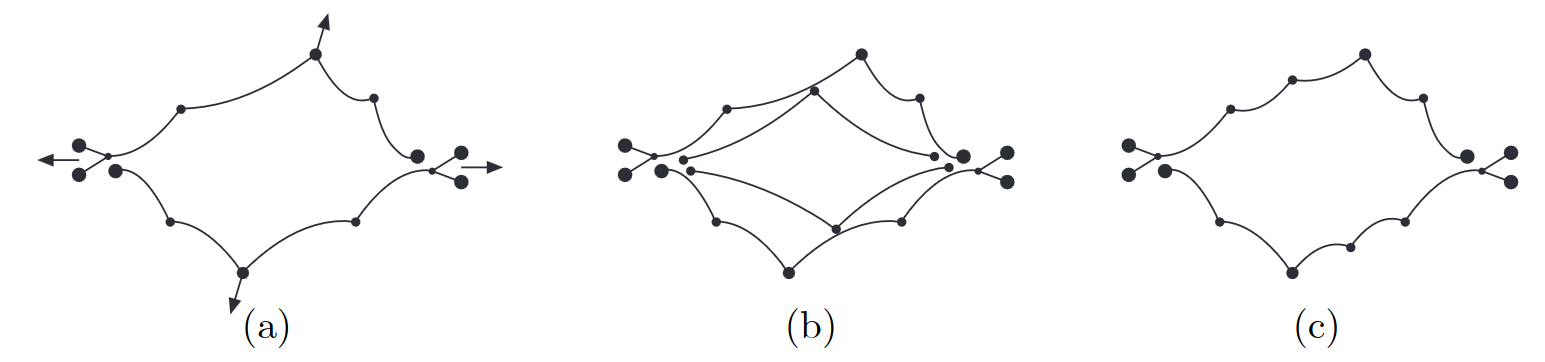
\includegraphics[height=7em]{\imgpath/cr.png}
\caption{Depiction of the CR process: \textbf{(a)} in a hard parton subcollision, the outgoing gluons are connected to the beam remnants through colour. Additional gluon kinks may occur through initial state radiation, which are ordered by rapidity. \textbf{(b)} A second hard scattering should theoretically result in two new strings connected to the remnants. \textbf{(c)} In order to minimise the total string length, gluons are colour reconnected. \cite{gustafsonMultipleInteractionsSaturation2009}}
\label{fig:intro:cr}
\end{figure}

It is also worth noting that the \pt boost acquired through color reconnection may depend on mass and whether a hadron is a baryon or meson, which somewhat mimics the hydrodynamic signatures of collective flow observed in AA collisions \cite{ortizColorReconnectionFlowlike2013}.

\section{Underlying event}\label{sec:intro:ue}

The underlying event (UE) in high-energy collisions refers to the additional hadronic activity that accompanies the primary hard scattering process, but is not directly related to it. This includes the fragmentation products of the beam remnants, ISR and FSR, as well as the effects of the previously discussed MPIs, and is visualised in Fig.~\ref{fig:intro:ue}. The UE (with its name coined at Tevatron \cite{cdfcollaborationChargedJetEvolution2002}) is typically characterized by a distribution of softer particles around and far outside of the hard process and was first observed at $\mathrm{Sp\bar{p}S}$ in the 1980s \cite{arnisonHadronicJetProduction1983}. These measurements saw a constant plateau of transverse energy $E_\mathrm{T}$ outside of the jet core, with its height independent of the jet energy.

\begin{figure}[H]
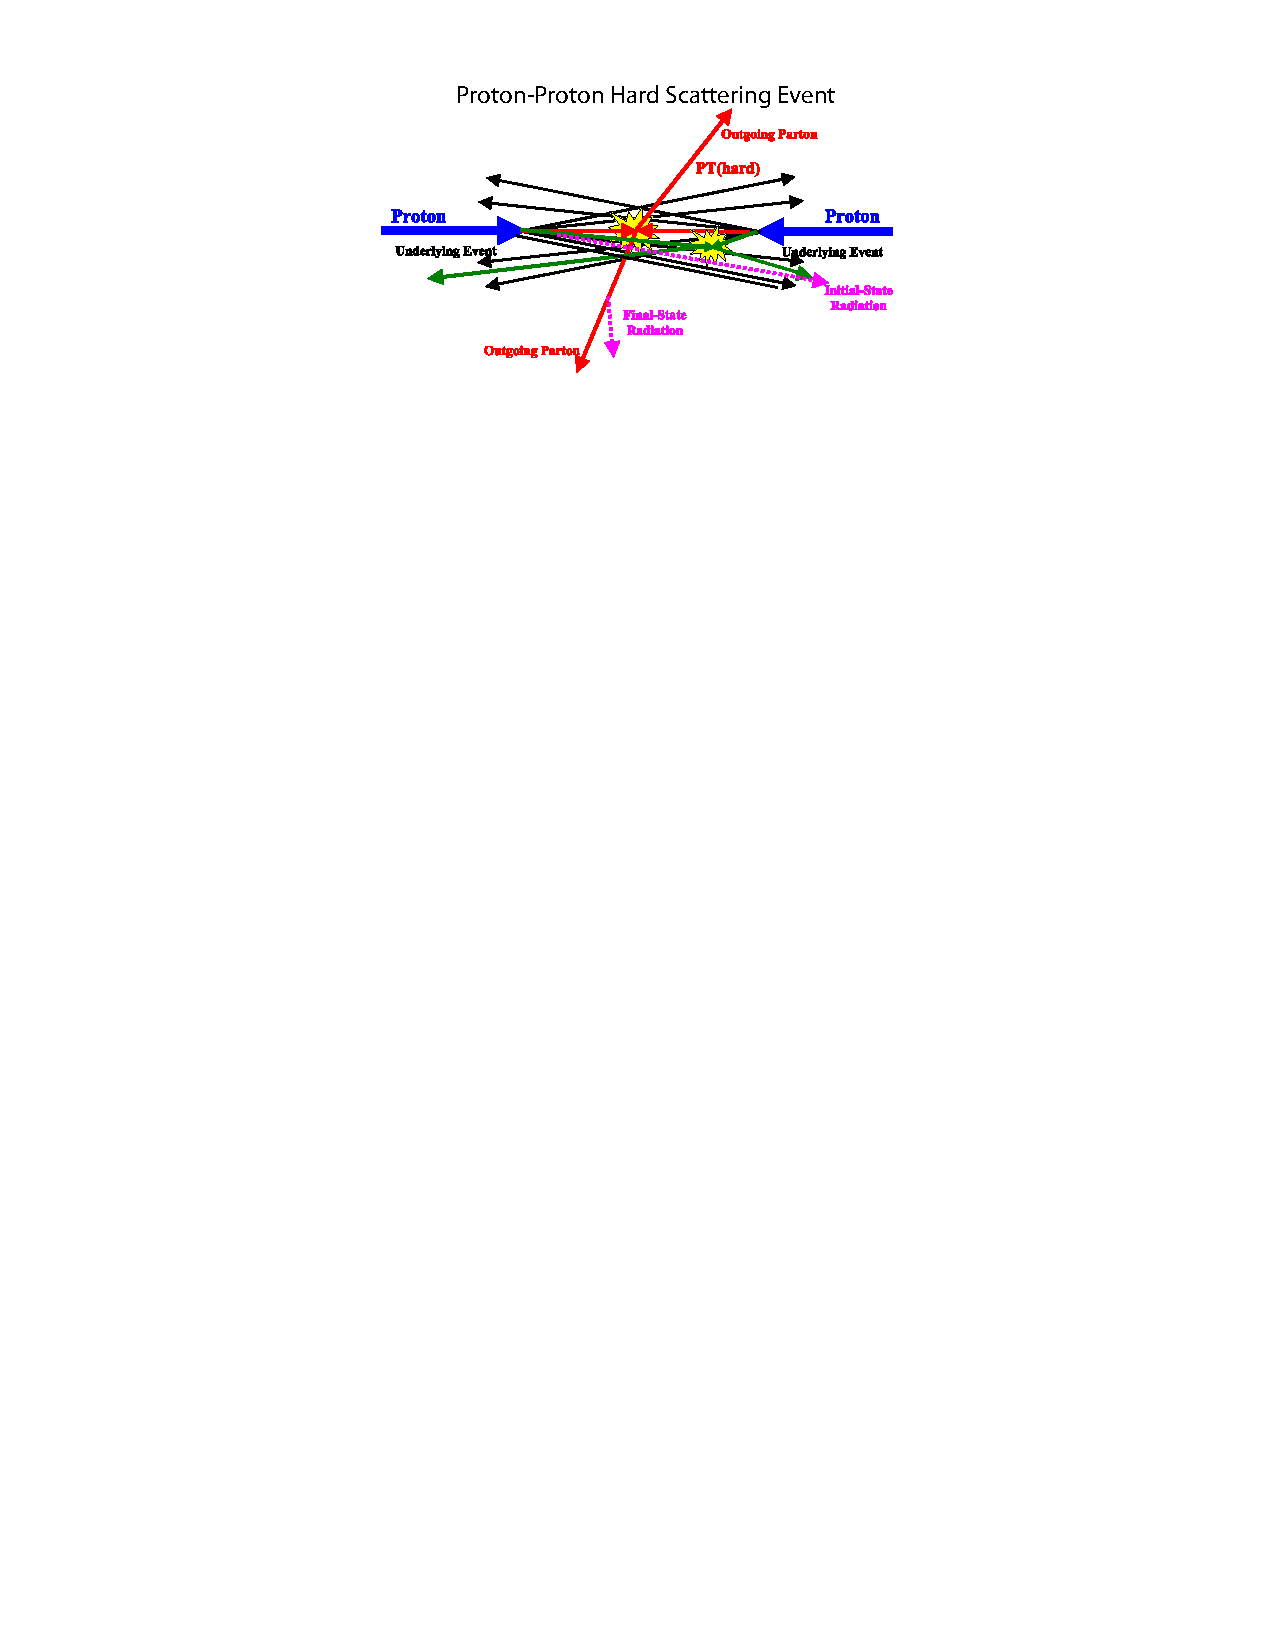
\includegraphics[width=.7\textwidth]{\imgpath/ue.pdf}
\caption{Cartoon illustrating a pp collision and its components: the hard scattering process, beam remnants, initial/final state radiation, and the MPIs. The last three contribute to the underlying event. \cite{cainesUnderlyingEventStudies2009, cdfcollaborationChargedJetEvolution2002}}
\label{fig:intro:ue}
\end{figure}

It is important to note that particle production in UE is different from the MB production, as it is biased by the presence of hard scattering. Additionally, the magnitude of the UE can fluctuate significantly from event to event.

\section{From hadrons to partons: deconfined QCD matter}

A simple argument can be made that confinement of quarks inside hadrons cannot be sustained when the density of partons is too large compared to that inside ordinary hadrons. Or alternatively, when the partonic kinetic energies are much larger than the confining part of the $q\bar{q}$ potential in (\ref{eq:intro:qqpot}). The following sections introduce some theoretical frameworks predicting the deconfinement of quarks and gluons. The calculations presented use natural units ($\hbar = c = k_B = 1$).

\subsection{Bag model of hadrons}

In this very naive approach \cite{detarBAGMODELSHADRONS1983, matonohaUpsilonMesonProduction2018}, hadrons are treated as spherical cavities (``bags") with radius $R$ of free massless quarks. These cavities exist in the non-perturbative QCD vacuum, which exerts a confining pressure $B$. The lowest-energy solution of the Dirac equation for the quarks, which in this case is $\slashed p \psi = 0$, is the $s_{1/2}$-state given by:
\begin{align}
\psi (r, t) = N \begin{pmatrix} j_0(\omega r) U \\ i \sigma \cdot \hat{r} j_1(\omega r) U \end{pmatrix} \exp (-i \omega t) \quad ,
\end{align}
where $N$ is a normalisation constant, $j_0$ and $j_1$ are spherical Bessel functions, $\omega$ is the quark energy, and $U$ the two-component spinor. The assumption that quarks are confined within the cavity volume represents the boundary conditions that the quark scalar density $\psi \bar{\psi}$ becomes zero at $r=R$, which is equivalent to $j_0(\omega R) = j_1(\omega R)$:
\begin{align}
j_0^2(\omega R) - \vec{\sigma} \cdot \hat{r} \vec{\sigma} \cdot \hat{r} j_1^2(\omega R) = 0 \\
j_0(\omega R) = j_1(\omega R) \quad ,
\end{align}
which happens when $\omega \approx \frac{2.04}{R}$. Thus, energy of the system can be given by
\begin{align}
E(R) \approx n_q \cdot \frac{2.04}{R} + \frac{4\pi}{3} B R^3 \quad .
\end{align}
Here, the first term represents the kinetic energy of $n_q$ quarks in the cavity and second term is the cavity volume energy. Gluon solutions should also be considered but are neglected in this approach. The first term acts to expand the cavity, whereas the second term acts to contract it. Finding an optimum of this energy with respect to $R$ leads to
\begin{align}\label{eq:intro:bagp}
B^{1/4} \approx \left( \frac{2.04 n_q}{4\pi} \right)^{1/4} \frac{1}{R} \quad .
\end{align}
Finally, assuming values for a proton, $R\approx 0.8$~fm, and three valence quarks $n_q=3$, the confining pressure can be approximated as $B^{1/4} \approx 206$~MeV. \cite{detarBAGMODELSHADRONS1983}

To relate the confining pressure to a critical temperature at which deconfinement occurs, $T_c$, one can assume a gas of relativistic massless fermions and bosons with energy density $\rho$ \cite{wongIntroductionHighEnergyHeavyIon1994, mcgreevyLectureNotesQuantum}. Using Stefan-Boltzmann law, the equation of state is,
\begin{equation}
P = \frac{1}{3} ( d_b + \frac{7}{8} d_f ) \rho = ( d_b + \frac{7}{8} d_f ) \frac{\pi^2}{90} T^4 \,
\end{equation}
where $d_b$ and $d_f$ are the degeneracy numbers for bosons and fermions, in this case gluons and quarks, respectively. Summing together possible colours, polarisations, and flavours for particles and antiparticles, one gets $d_b = 16$ and $d_f = 24$. Inserting the cavity pressure $B$ value calculated in (\ref{eq:intro:bagp}), $T_c$ can be estimated as approximately $145$~MeV.

\subsection{Lattice QCD}

Lattice QCD (LQCD) is a technique allowing calculation of processes involving the strong interaction in the non-perturbative regime, from first principles, without phenomenological assumptions. In this approach, the space-time continuum is discretised into a four-dimensional lattice, which allows QCD path integrals to be solved numerically. Smallest squares on the lattice are called \textit{plaquettes}, with the lattice links representing gluon fields and lattice sites representing quark fields. \cite{meyerLatticeQCDBrief2015}

Lattice calculations are computationally extremely intensive\footnote{In fact, in the past, LQCD was among important drivers of the advancement of GPU computing and it is also used as benchmark in high-performance computing \cite{bennettBSMBenchFlexibleScalable2016}.}, thus, a sufficiently coarse lattice spacing must be chosen to reduce computational costs and make the approach feasible. Often, simulations are also performed with unphysical quark masses (e.g.\ $m_q \sim m_\pi$), for the same reason. The results are then extrapolated using highly complex methods. Another limitation in LQCD is the so-called \textit{sign problem}, discussed in detail for instance in Ref.~\cite{nagataFinitedensityLatticeQCD2022}, which arises when evaluating highly oscillatory complex integrals in finite-density environment.

Despite its challenges, LQCD has been successful in various predictions, notably, the \textit{ab initio} calculation of the mass of neutron (uud) using the mass of $\Omega$ (sss) as an input \cite{durrInitioDeterminationLight2008}. Furthermore, it allows for the calculation of thermodynamics of QCD matter and predicts its equation of state, as well as a phase transition at $T_c \approx 150$~MeV \cite{petreczkyLatticeQCDNonzero2012, bazavovEquationStateFlavor2014}, which is usually identified with the formation of quark-gluon plasma QGP, discussed in Chapter~\ref{chap:colls}. The dependence of energy density and pressure on temperature can be seen in Fig.~\ref{fig:intro:eos}.

\begin{figure}[H]
\subfloat[][]{\adjustbox{valign=m}{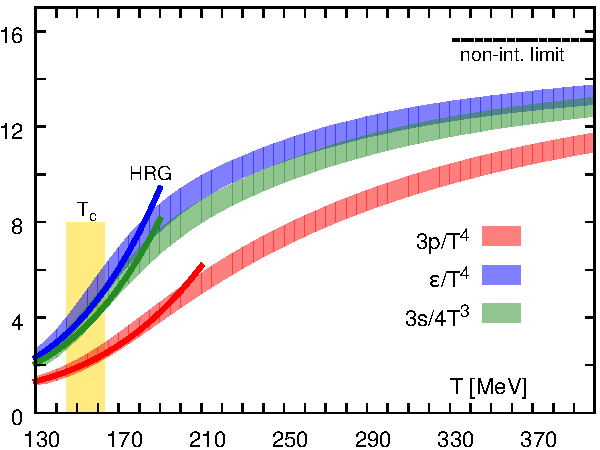
\includegraphics[width=.40\textwidth]{\imgpath/eos.pdf}}}\hspace{1.5em}%
\subfloat[][]{\adjustbox{valign=m}{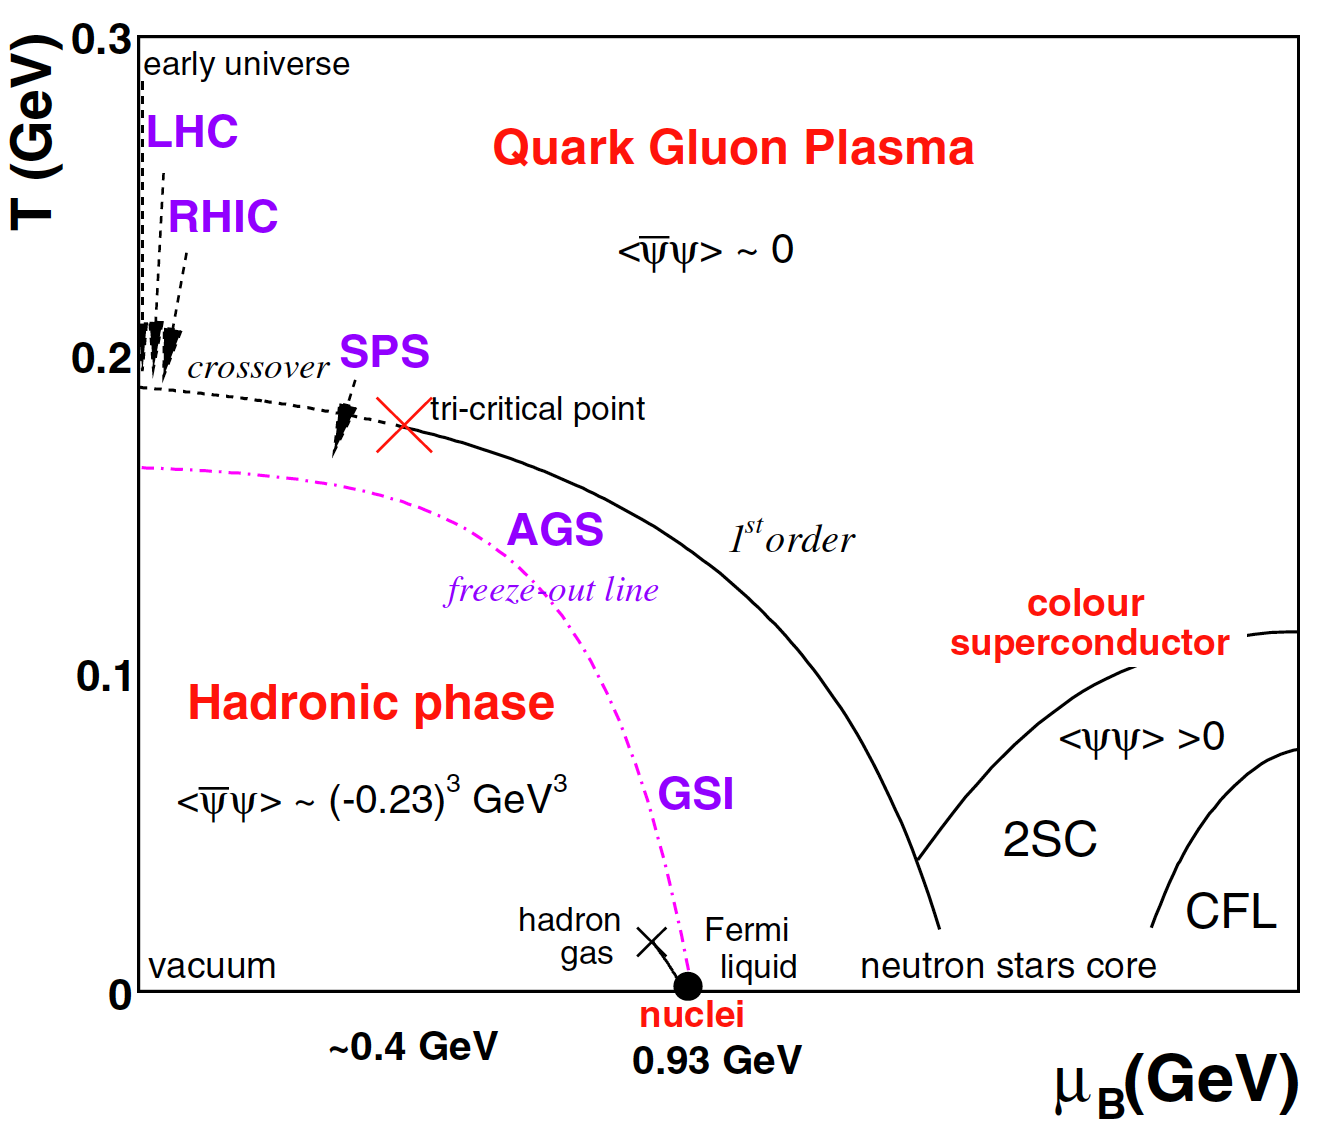
\includegraphics[width=.50\textwidth]{\imgpath/phasediagram.png}}}
\caption{\textbf{(a)} Dependence of the pressure (red), energy density (blue), and entropy density (green) on temperature, determined with LQCD. \cite{bazavovEquationStateFlavor2014} \textbf{(b)} Phase diagram of QCD matter. \cite{pasechnikPhenomenologicalReviewQuark2017}}
\label{fig:intro:eos}
\end{figure}

\subsection{QCD phase diagram, chiral symmetry restoration}

Phase transitions of QCD matter are investigated to explore the QCD phase diagram with respect to temperature $T$ and baryon chemical potential $\mu_B$, which corresponds to net baryon density. Figure~\ref{fig:intro:eos} visualizes the different areas of the QCD phase diagram probed by various experiments \cite{pasechnikPhenomenologicalReviewQuark2017}. Measurements of Pb-Pb collisions at the LHC access high $T$ and almost zero $\mu_B$, as the nucleons of ultrarelativistic Pb nuclei escape the interaction volume before the plasma develops, and the high energy subsequently leads to a sizable baryon production balanced by anti-baryons due to conservation laws. Experiments studying collisions of slower and heavier nuclei reach higher $\mu_B$ regions.

Furthermore, looking back at the QCD Lagrangian in (\ref{eq:intro:lqcd}) and neglecting quark current masses $m_{u,d}\to 0$, it can be seen that it is invariant when switching the up and the down quark, corresponding to a SU($2$) isospin symmetry. This allows the fermion fields to be rewritten in terms of their left and right chiralities and the QCD Lagrangian then exhibits a larger \textit{chiral symmetry}.

However, it is known that the vacuum expectation value of a $q\bar{q}$ state is much larger than the current masses $m_{u,d}$:
\begin{equation}
\langle 0 | q \bar{q} | 0 \rangle = \langle 0 | u\bar{u} + d \bar{d} | 0 \rangle \approx (250 \, \mathrm{MeV} )^3 \quad ,
\end{equation}
where the value is taken from average masses of light flavour mesons. This means that the QCD vacuum spontaneously breaks the chiral symmetry. \cite{sazdjianIntroductionChiralSymmetry2017}

It can be expected that in the plasma of deconfined quarks and gluons, chiral symmetry is \textit{restored} \cite{gottliebEstimatingChiralsymmetryRestoration1987, xuChiralSymmetryRestoration2023}. This is actively studied in AA collisions, for example in searches of the so-called chiral magnetic effect \cite{starcollaborationSearchChiralMagnetic2021} or degeneracy of normally chiral partners \cite{hohlerRmesonMeltingCompatible2014}, such as the $\rho$ ($J^P=1^-$) and $a_1$ ($J^P=1^+$) states.

%\section{Implications of high-activity QCD research}
%
%Understanding the early universe: The QGP is believed to have existed in the first few microseconds after the Big Bang. Studying QGP can provide insight into the behavior of matter and the formation of the universe
%Understanding of fundamental physics: QGP is a unique state of matter that is not well understood. Studying QGP can provide insight into the behavior of quarks and gluons, which are the building blocks of matter.
%Developing a deeper understanding of strong interactions: The strong nuclear force is one of the four fundamental forces of nature. Studying QGP can provide insight into the behavior of this force and its interactions with matter.